
\section{Prädikatenlogik: Semantik}

\begin{frame}[t]{Interpretationen}
	\begin{block}{Interpretation $(D,I)$}
		\begin{itemize}
			\item nichtleere Menge $D$ \quad „Universum“
			\item $I(\word c_i) \in D$
			\item $I(\word f_i) \from D^k \functionto D$ \quad ($k$: Stelligkeit von $\word f_i$)
			\item $I(\word R_i) \subseteq D^k$ \; Relation auf D \quad ($k$: Stelligkeit von $\word R_i$)
			\item \textbf{KEINE} Werte für Variablen!
		\end{itemize}
		Beispiel: \\
		\only<all:1>{
			\begin{itemize}
				\item $D = \N_0$
				\item $I(c) = 42$
				\item $\ar(\word f) = 1$, \\ $I(\word f) \from \N_0 \functionto \N_0, \, I(\word f)(n) = n+2$
				\item $\ar(\word R) = 2$, \; $I(\word R) = \set{(n, m) \Mid 2n \geq m }$ 
			\end{itemize}
		}
		\visible<all:2>{
			\begin{itemize}
				\item $D = \text{Alle Menschen} \cup \text{Alle Namen}$
				\item $I(\word{knuth}) = \text{Donald E. Knuth}$
				\item $\ar(\word{vorname}) = 1$, \\ $I(\word {vorname}) \from D \functionto D, \, I(\word {vorname})(\text{Donald E. Knuth}) = \word{Donald}$, ....
				\item $\ar(\word {bekannt}) = 1$, \; $I(\word {bekannt}) = \set{\text{Donald E. Knuth, Donald Trump, ...}}$
			\end{itemize}
		}
	\end{block}
\end{frame}

\begin{frame}{Variablenbelegungen, Auswertung}
	\begin{block}{Variablenbelegung $\beta \from \VPL \functionto D$}
		Mehrere verschiedene für eine feste Interpretation $(D,I)$ möglich! \\
		Beispiel: \\
		\begin{itemize}
			\item $\beta(\word x) = 42, \beta(\word y) = 1337$ \quad oder
			\item $\beta(\word x) = 2, \beta(\word y) = 10000$ 
		\end{itemize}
	\end{block}
	\pause
	\begin{block}{Auswertung}
		$\valDIb$ \quad „Auswertungsfunktion“ \\
		\begin{itemize}
			\item rechnet Werte aus für Terme \\
			$\valDIb(\word x) = 42$, \; $\valDIb(\word{f(y)}) = 1337 + 2 = 1339$
			\item rechnet Wahrheitswerte aus für ganze PL-Formeln \\
			$\valDIb(\plexists \word n \, \plka\word{prim(n)\plkz}) = \W$, \; $\valDIb(\plall \word m \, \plka \word{vorname(m)}\pleq \word{Donald} \plkz) = \F$
			\item „wie wir's kennen“
		\end{itemize}
	\end{block}
\end{frame}

\mycomment{
	\begin{frame}{Interpretation}
		\begin{figure}[h!]
			\centering
			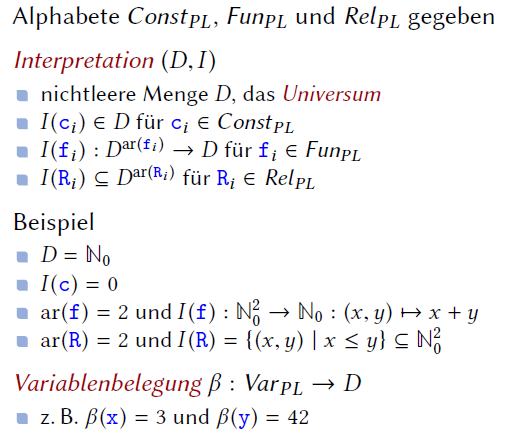
\includegraphics[scale=0.6]{pl/int.png} \hspace{2em} 
		\end{figure} 
	\end{frame}
}

\begin{frame}{Aufgabe}
	\[ F := \plexists \plx {\plka \word{f(x)} \pleq \plx \aland \plx \pleq \ply \plkz}  \]
	
	Gebt eine Interpretation $(D_1, I_1)$, $D \nsubseteq \R$, und eine Variablenbelegung $\beta_1$ so an, dass $val_{D_1, I_1, \beta_1}(F) = \W$ gilt.\\
	\smallskip
	\visible<2-|handout:2>{Die Interpretation $(D_1, I_1)$ mit $ D_1 = \{ \word a, \word b \}^*, \, I_1(\word f)(w) = \word a$ und die Variablenbelegung $\beta_1 \colon \VPL \functionto D_1$, $v \mapsto \word a$, tun es.} \\
	\medskip
	
	\[ G := \alnot\word{S(z)} \aland \plexists \plx {\plka \word{S(x)} \aland \plall \ply \word{R(x,y)} \plkz}  \]
	
	Gebt eine Interpretation $(D_2, I_2)$, $D \subseteq \N$, und eine Variablenbelegung $\beta_2$ so an, dass $val_{D_2, I_2, \beta_2}(G) = \W$ gilt.\\
	\smallskip
	\visible<3-|handout:2>{Die Interpretation $(D_2, I_2)$ mit $ D_2 = \set{0, ..., 5}, \, I_2(\word S) = \set{n \Mid \text{$n$ ist prim}}, I_2(\word R) = {\geq} $ und die Variablenbelegung $\beta_2 \colon \VPL \functionto D_2$, $\plz \mapsto 4, \, \text{...Rest beliebig...}$, tun es.}
	
\end{frame}

\begin{frame}{Aufgabe 1 (WS 15/16, Blatt 7)}
	  \begin{equation*}
	F = \alnot \plexist \plx
	{\plka
		\plE{\plka \plx \plcomma \ply \plkz}
		\alor
		\alnot \plall \plz \plall \plx \plall \ply
		{\plka
			\plE{\plka \plx \plcomma \plz \plkz} \aland \plE{\plka \ply \plcomma \plz \plkz} \alimpl \plx \pleq \ply
			\plkz}
		\plkz}
	\end{equation*}\\[1em]
	
	\begin{block}{Aufgabe 1.3}
		Gebt eine Interpretation $(D_1, I_1)$ und eine Variablenbelegung $\beta_1$ so an, dass $val_{D_1, I_1, \beta_1}(F) = \W$ gilt.\\[0.5em]
		
		\visible<2-|handout:2>{Die Interpretation $(D_1, I_1)$ mit $ D_1 = \{ 0, 1 \}, \, I_1(\word E) = {<}$ und die Variablenbelegung $\beta_1 \colon \VPL \functionto D_1$, $v \mapsto 0$, tun es.}
	\end{block}

	\begin{block}{Aufgabe 1.4}
		Gebt eine Interpretation $(D_2, I_2)$ und eine Variablenbelegung $\beta_2$ so an, dass $val_{D_2, I_2, \beta_2}(F) = \F$ gilt.\\[0.5em]
		
		\visible<3-|handout:2>{Die Interpretation $(D_2, I_2)$ mit $ D_2 = \{ 0, 1 \}, \, I_2(\word E) = {<}$ und die Variablenbelegung $\beta_2 \colon \VPL \functionto D_2$, $v \mapsto 1$, tun es.}
	\end{block}
\end{frame}

\section{Prädikatenlogik: Aufgaben}

\begin{frame}{Prädikatenlogische Formeln aufstellen}
	% TODO Aufgaben!
	Vgl. Übung WS 15/16
\end{frame}